\begin{table*}[t]
\centering
\begin{tabular}{lc|cccc|c}
\hline
\textbf{Method}                     & \textbf{Gr. Sup.}& \multicolumn{4}{|c|}{\textbf{CV-Bench \& PixCV-Bench}} \\
                                    &                  & $\mathcal{A}\dagger$  & $\mathcal{A}$ & $\mathcal{M}$ & $\mathcal{M}\dagger$ & $\mathcal{S}$\\\hline
LLava 1.5 (7B)                      & \xmark           & \textbf{52.6/66.2/59.4} & \textbf{55.0/67.5/61.3} &     -     &     -      & -\\
LLava 1.5 (13B)                     &  \xmark          & \textbf{51.8/65.6/59.1} & \textbf{55.6/68.7/62.1} &     -     &    -       & -\\
Cambrian (8B)*~\cite{tong2024cambrian}&\xmark          & \textbf{64.5/77.4/71.0} & \textbf{65.1/79.4/72.3} &     -     &     -   & -\\
%OMG LLava (7B)                       &   \checkmark   &  32.2/36.4/34.3 & 36.8/47.4/42.1 &          &           & \\%GPT:rawQs
OMG LLava (7B)                       &   \checkmark    & 36.5/46.3/41.4 & 36.8/47.4/42.1 &   -       &   51.0  & \textbf{46.6}\\%GPT:CVBenchQs
GLAMM (7B)                        &    \checkmark   &      -         &      -         &  \textbf{30.2}     &   \textbf{52.4}    & -\\
%GLAMM - RegCap                       &   \checkmark    & 43.8/55.3/49.6 & 46.8/62.0/54.4 &  3.6      &  7.9      & \\%GPT:rawQs
GLAMM - RegCap (7B)                      &   \checkmark    & 46.6/61.6/54.1 & 46.8/62.0/54.4 &  3.6      &  7.9  & 31.2\\%GPT:CVBenchQs
LISA (7B)                            &   \checkmark    & 8.4/16.4/12.4  &       -        &   16.8    &  47.9     & 30.2\\
LLava-G (7B)                         &    \checkmark   & 32.7/37.8/35.3 & 5.1/3.7/4.4    &    1.7    &  18.6     & 27.0\\%GPT:rawQs
%LLava-G (7B)                         &    \checkmark   & 31.8/35.8/33.7 & 5.1/3.7/4.4    &           &          &\\%GPT:CVBenchQs
LLava 1.5 (7B) + (a+s)               & \xmark          & \textbf{52.6/66.2/59.4} & \textbf{55.0/67.5/61.3} &   4.7     &    14.9   & 38.5\\ 
LLava 1.5 (13B) + (a+s)              & \xmark          &  \textbf{51.8/65.6/59.1} & \textbf{55.6/68.7/62.1} &    5.2    &   15.7    & 38.5\\ 
Cambrian (8B)* + (a+s)~\cite{cao2024emerging}  & \xmark & \textbf{64.5/77.4/71.0} & \textbf{65.1/79.4/72.3} &  18.5    &   15.9    &  \textbf{45.4}\\ \hline %19.3
PixFoundation (LLava (7B)) (Ours)    & \xmark          & \textbf{52.6/66.2/59.4} & \textbf{55.0/67.5/61.3} &    5.0     &    18.7   & 40.0\\ 
PixFoundation (LLava (13B)) (Ours)   & \xmark          & \textbf{51.8/65.6/59.1} & \textbf{55.6/68.7/62.1} &    4.7     &     18.4  & \textbf{40.3}\\ 
PixFoundation (Cambrian (8B)*)(Ours)  & \xmark         & \textbf{64.5/77.4/71.0} & \textbf{65.1/79.4/72.3} &    11.8     &     16.1  & 44.2\\ \hline
\multicolumn{7}{l}{\textbf{Upper Bound - Oracle Selection}} \\ \hline
PixFoundation$\dagger$ (LLava (7B)) (Ours)    & \xmark  & 52.6/66.2/59.4 & 55.0/67.5/61.3 &    \textcolor{red}{\textbf{6.3}}    &     \textcolor{red}{\textbf{49.7}}  & \textcolor{red}{\textbf{55.5}}\\ 
PixFoundation$\dagger$ (LLava (13B)) (Ours)    & \xmark & 51.8/65.6/59.1 & 55.6/68.7/62.1 &    \textcolor{red}{\textbf{5.3}}    &     \textcolor{red}{\textbf{51.7}}  & \textcolor{red}{\textbf{56.9}}\\ 
PixFoundation$\dagger$ (Cambrian (8B)*) (Ours)  & \xmark & 64.5/77.4/71.0 & 65.1/79.4/72.3 &   \textcolor{red}{\textbf{54.6}}   &   \textcolor{red}{\textbf{64.5}}   &  \textcolor{red}{\textbf{68.4}}\\ \hline 
\end{tabular}
\caption{Evaluation of the various pixel-level MLLMs and the different baselines on PixCV-Bench benchmark. We evaluate the visual question answering accuracy and accuracy using GPT-4o in the first two protocols (i.e., $\mathcal{A}, \mathcal{A}\dagger$ resp.). Note, we show the accuracies as $././.$ as the ADE20K, COCO and average of both respectively. Additionally, we evaluate pixel-level visual grounding ability with output segmentation masks in the first and third protocols (i.e., $\mathcal{M}, \mathcal{M}\dagger$ resp.). *: models using Llama 3 (8B) unlike the rest that are relying on Vicuna (7B and 13B) for the base LLM. - : indicates either the model can not be evaluated in that setting, or has low results below 1\% showing complete failure in that setting. $\mathcal{S}$: denotes the score of the MLLM that is average of $\text{max}(\mathcal{A}, \mathcal{A}\dagger)$ and $\text{max}(\mathcal{M}, \mathcal{M}\dagger)$.  The oracle results are highlighted in red, and the best in each variant (7B, 13B, and 8B) are bolded.}
\label{tab:pixcvbench}
\end{table*}

\begin{figure*}[t]
\centering
the dorsal fin of the animal

\begin{subfigure}{0.19\textwidth}
\includegraphics[width=\textwidth]{images/qualfig1/OMGLLava/output00019.png}
\end{subfigure}%
\begin{subfigure}{0.19\textwidth}
\includegraphics[width=\textwidth]{images/qualfig1/LISA/output00019.png}
\end{subfigure}%
\begin{subfigure}{0.19\textwidth}
\includegraphics[width=\textwidth]{images/qualfig1/GLAMM/output00019.png}
\end{subfigure}%
\begin{subfigure}{0.19\textwidth}
\includegraphics[width=\textwidth]{images/qualfig1/LLava-G/19.jpg}
\end{subfigure}%
\begin{subfigure}{0.19\textwidth}
\includegraphics[width=\textwidth]{images/qualfig1/LLava157b/19.jpg}
\end{subfigure}

the butterfly's feet 

\begin{subfigure}{0.19\textwidth}
\includegraphics[width=\textwidth]{images/qualfig1/OMGLLava/output00107.png}
\caption{}
\end{subfigure}%
\begin{subfigure}{0.19\textwidth}
\includegraphics[width=\textwidth]{images/qualfig1/LISA/output00107.png}
\caption{}
\end{subfigure}%
\begin{subfigure}{0.19\textwidth}
\includegraphics[width=\textwidth]{images/qualfig1/GLAMM/output00107.png}
\caption{}
\end{subfigure}%
\begin{subfigure}{0.19\textwidth}
\includegraphics[width=\textwidth]{images/qualfig1/LLava-G/107.jpg}
\caption{}
\end{subfigure}%
\begin{subfigure}{0.19\textwidth}
\includegraphics[width=\textwidth]{images/qualfig1/LLava157b/107.jpg}
\caption{}
\end{subfigure}
\caption{Qualitative comparison on PixMMVP between the pixel-level visual grounding following the third evaluation protocol. (a) OMG-LLava, (b) LISA, (c) GLAMM, (d) LLava-G, (e) PixFoundation$\dagger$ (7B) oracle baseline. The referred expression used in the segmentation is shown on top of each row. It shows persistently that mining for the grounding within attention maps of MLLMs that were not trained with grounding supervision and doing the oracle selection outperforms the pixel-level MLLMs trained with full grounding supervision. It clearly shows the oracle excels in identifying fine-grained object parts and descriptions that other pixel-level MLLMs are not necessarily capable of. The second best performance is GLAMM yet we showed it is completely incapable of performing visual question answering unless fine-tuned for the region captioning task at which then some of its gronuding ability is lost.} 
\vspace{-0.5em}
\label{fig:qual}
\end{figure*}

\begin{figure*}[t]
\centering
\begin{subfigure}{0.48\textwidth}
\begin{tikzpicture}
\begin{axis} [
     title={},
     width=\textwidth,
     height=.2\textheight,
     xlabel={\footnotesize \textbf{Location}},
     ylabel={\footnotesize \textbf{Frequency}},
     bar width = 4pt,
     ybar = .02cm,
     xmin=-5, xmax=100,
     ymin=0.0, ymax=80,
     x tick label style={font=\tiny},
     y tick label style={font=\tiny},
     xtick={0, 10,20,30,40,50,60,70,80,90},
     y label style={at={(axis description cs:0.05,.5)},anchor=south},
     ymajorgrids=false,
     xmajorgrids=false,
     legend style={
			at={(0.5,-0.35)},
			anchor=north,
			legend columns=5,
            }
] 

%{0: 31, 1: 9, 2: 15, 3: 24, 4: 27, 5: 27, 6: 50, 7: 28, 8: 29, 9: 7}
\addplot[color=red, fill=red,  area legend] coordinates {(0, 31) (10, 9) (20, 15) (30, 24) (40, 27) (50, 27) (60, 50) (70, 28) (80, 29) (90, 7)};

%{0: 29, 1: 6, 2: 15, 3: 29, 4: 18, 5: 35, 6: 41, 7: 37, 8: 29, 9: 8}
\addplot[color=red!50, fill=red!50,  area legend] coordinates {(0, 29) (10, 6) (20, 15) (30, 29) (40, 18) (50, 35) (60, 41) (70, 37) (80, 29) (90, 8)};

%{0: 23, 1: 29, 2: 30, 3: 29, 4: 31, 5: 30, 6: 30, 7: 23, 8: 12, 9: 10}
\addplot[color=blue, fill=blue,  area legend] coordinates {(0, 23) (10, 29) (20, 30) (30, 29) (40, 31) (50, 30) (60, 30) (70, 23) (80, 12) (90, 10)};

\legend{\textbf{Llava (7B)}, \textbf{Llava (13B)},\textbf{Cambrian (8B)}}
  
\end{axis}
\end{tikzpicture}
\caption{}
\label{fig:tokenloc}
\end{subfigure}%
\begin{subfigure}{0.52\textwidth}
\begin{tikzpicture}
\begin{axis} [
     title={},
     width=\textwidth,
     height=.2\textheight,
     xlabel={\footnotesize \textbf{Concept}},
     ylabel={\footnotesize \textbf{Frequency}},
     bar width = 4pt,
     ybar = .02cm,
     xmin=0, xmax=7,
     ymin=0.0, ymax=200,
     xtick=data,
     x tick label style={font=\tiny,align=center},
     y tick label style={font=\tiny},
     xtick={1,2,3,4,5,6},
     xticklabels={{Colour \& \\ Appearance}, {Location \& \\ Position}, {Objects \\ Parts}, {Context}, {Objects \&\\Entities}, {State}},
     y label style={at={(axis description cs:0.05,.5)},anchor=south},
     x label style={at={(axis description cs:0.5,-.07)},anchor=north},
     ymajorgrids=false,
     xmajorgrids=false,
     legend style={
			at={(0.5,-0.45)},
			anchor=north,
			legend columns=5,
            }
] 

%{'a': 32, 'b': 21, 'c': 37, 'd': 19, 'e': 144, 'f': 3}
\addplot[color=red, fill=red,  area legend] coordinates {(1, 32) (2, 21) (3, 37) (4, 19) (5, 144) (6, 3)};

%{'a': 35, 'b': 16, 'c': 38, 'd': 17, 'e': 143, 'f': 3}
\addplot[color=red!50, fill=red!50,  area legend] coordinates {(1, 35) (2, 16) (3, 38) (4, 17) (5, 143) (6, 3)};

%{'a': 36, 'b': 15, 'c': 56, 'd': 2, 'e': 114, 'f': 25}
\addplot[color=blue, fill=blue,  area legend] coordinates {(1, 36) (2, 15) (3, 56) (4, 2) (5, 114) (6, 25)};

\legend{\textbf{Llava (7B)}, \textbf{Llava (13B)},\textbf{Cambrian (8B)}}
  
\end{axis}
\end{tikzpicture}
\caption{}
\label{fig:tokenconcept}
\end{subfigure}
\caption{Analysis on when does grounding emerge on PixMMVP benchmark using the three base MLLMs that were not trained with grounding supervision and following the third evaluation protocol then reporting the oracle selection. (a) Analysis on the output token location that coincides with the best segmentation mask. (b) Analysis on the output token concept category that coincides with the best segmentation mask..}
\label{tab:When_MMVP}
\end{figure*}

\subsection{Experimental Setup}

\textbf{Evaluation benchmarks, protocols and metrics.}
We rely on the publicly released MMVP~\cite{tong2024eyes} augmented with our annotations that is composed of 300 images paired with questions, choices, referring expressions and segmentation masks, which we call PixMMVP. Additionally, we augment CV-Bench~\cite{tong2024cambrian} 2D with our annotations resulting in 1,438 images with their corresponding questions, choices, referring expressions and segmentation masks. On each benchmark we evaluate the visual question answering and visual grounding capabilities following three protocols. First protocol, we prompt the model using the question and choices directly. We then evaluate the accuracy using GPT-4o following previous work~\cite{tong2024eyes} reported as, $\mathcal{A}\dagger$. Additionally, if the model generates a segmentation mask without an explicit request for that segmentation, the model is evaluated with respect to the ground-truth referring segmentation in terms of mean intersection over union reported as, $\mathcal{M}$. The second protocol, we follow previous work~\cite{tong2024cambrian} in prompting the models with the question, choices and an explicit instruction to output a single option letter. The accuracy for the visual question answering is evaluated directly without the need for GPT-4o and reported as, $\mathcal{A}$. There is a need for the first protocol since some of the recent pixel-level MLLMs face challenges in following instructions and are incapable of outputting a single option letter. The third protocol prompts the MLLMs to output a segmentation mask of the referred object and evaluate mean intersection over union reported as, $\mathcal{M}\dagger$. We evaluate the score of each model, $\mathcal{S}$, which is the average performance across the maximum of both pixel-level visual grounding and visual question answering (i.e., average of $\text{max}(\mathcal{A}, \mathcal{A}\dagger)$ and $\text{max}(\mathcal{M}, \mathcal{M}\dagger)$). We mainly focus on evaluating four state-of-the-art pixel-level multi-modal large language models; LISA~\cite{lai2024lisa}, GLAMM~\cite{rasheed2024glamm}, OMG-LLava~\cite{zhang2024omg} and LLava-G~\cite{zhang2025llava}. Specifically, for GLAMM we use two variants; the original model (GLAMM) and the one fine-tuned for region captioning, (GLAMM-RegCap). Refer to Appendix~\ref{} for more details.%the detailed prompts used under the three protocols and the checkpoints used for each model variants from HuggingFace~\cite{wolf2019huggingface}.

\textbf{Baselines implementation details.} We evaluate our three baselines that rely on MLLMs that are not trained with pixel-level grounding which are: (i) the attend and segment (a+s), (ii) the oracle selection relying on the highest intersection over union in selecting the correctly predicted masks (PixFoundation$\dagger$), and (iii) the automatic selection detailed in Sec.~\ref{}, (PixFoundation). The three baselines are implemented on top of three base MLLMs which are, LLava 1.5 (7B, 13B)~\cite{liu2024improved} and Cambrian-1(8B)~\cite{tong2024cambrian}. The automatic selection is implemented using the Cambrian-1 (8B) model as an open source model, yet the automatic selection mechanism can be further improved by using GPT-4o. Refer to Appendix~\ref{} for the model checkpoints used for the three base MLLMs.

\subsection{Are the current pixel-level MLLMs trained with full grounding supervision heading in the right direction?}
In order to answer this question we evaluate each of these pixel-level MLLMs capability in visual question answering as a necessary capability for any multi-modal large language model. Additionally, we evaluate their ability to visually ground the objects of interest in these questions using the manually defined referring expressions. 

\textbf{PixMMVP Benchmark}
Table~\ref{tab:pixmmvp} shows the results of the four major pixel-level MLLMs on the challenging PixMMVP benchmark. From the accuracy of visual question answering multi-modal large language models that were never trained with pixel-level grounding supervision surpass their pixel-level counterpart with up to 15\%. The best model in pixel-level MLLMs in this aspect is OMG-Llava~\cite{zhang2024omg} that still shows good ability to follow instructions and conduct the standard task of visual question answering. On the other hand, when looking at pixel-level visual grounding we find the best model, GLAMM~\cite{rasheed2024glamm}, while surpassing all the other models has a weak ability in visual question answering or following instructions to output the correct option letter. Moreover, it shows certain models like LISA and LLava-G are incapable of following the instruction for outputting the correct option letter shown in, $\mathcal{A}$, although when prompted only with the question they can still show weak ability in visual question answering. Looking at the bottom three rows showing the baseline of mining the attention maps for the maximum attention point per output token to prompt SAM followed by using the oracle selection of the best predicted mask, it shows that MLLMs that were never trained with grounding supervision have the correct information within their learned attention maps. In fact looking at the final score, $\mathcal{S}$, for the oracle variant, PixFoundation$\dagger$ (7B), and the corresponding best pixel-level MLLMs, OMG-LLava (7B) and GLAMM (7B), the oracle outperforms both by a considerable margin while the automatic outperforms them with up to 3\%. While the attend and segment baseline~\cite{cao2024emerging} is showing competitive performance on PixMMVP it still lags behind our automatic selection method, and the oracle performance shows that all methods still lag behind the already existing information in MLLMs if just mined for with the correct scheme without any grounding supervision.

\textbf{PixCV-Bench Benchmark}
Table~\ref{tab:pixcvbench} shows the results of the same MLLMs on the 2D PixCV-Bench benchmark. Persistently all the pixel-level MLLMs still lag behind the MLLMs that were never trained with grounding supervision. Nonetheless, OMG-LLava strikes the right balance in both visual question answering and pixel-level visual grounding with the highest score, $\mathcal{S}$, within the 7B models. While, GLAMM, shows the best pixel-level visual grounding yet it is incapable of any visual question answering on this benchmark. Looking at the bottom three rows for the oracle in terms of the score $\mathcal{S}$, similar to our previous conclusions the simple mining for grounding within the attention maps of MLLMs that were never trained with grounding supervision still surpass all the pixel-level MLLMs. When looking at the attend and segment baseline and the automatic PixFoundation baseline, both lag behind the oracle as expected yet they show competitive performance in pixel-level visual grounding. Our automatic PixFoundation baseline outperforms the attend and segment using the Llava variants as base, while showing competitive performance using the Cambrian base model.

\textbf{Summary of findings.} In summary, we found that pixel-level MLLMs trained with full grounding supervision, when looking at the score $\mathcal{S}$, lag behind simple mining of grounding from the attention maps of MLLMs that were never trained with grounding when computing their upper bound (i.e., PixFoundation$\dagger$). Our conclusion that full grounding supervision does degrade their ability in visual question answer and instruction following and in certain models even their visual grounding is degraded. This is mainly occurring with challenging tasks like the PixMMVP benchmark. Moreover, it shows that the grounding that is emerging in our baselines does not necessarily coincide with the output token corresponding to the noun phrase that is most similar to the referred expression in our ground-truth. This is clearly conveyed in both benchmarks in how the Oracle upper bound surpasses the attend and segment baseline with considerable margins across all variants. We also show that our proposed automatic baseline provides an initial simple direction on how to automate the selection of the masks which outperforms the current state-of-the-art in the majority of the variants.

\subsection{When does grounding emerge in MLLMs?}

\begin{figure}[t]
\centering
\resizebox{0.3\textwidth}{!}{
\begin{tikzpicture}
\begin{axis} [
     title={},
     height=.2\textheight,
     xlabel={\tiny{\textbf{Oracle + Point Selection Variants}}},
     ylabel={\textbf{\tiny{$\mathcal{M}$}}},
     bar width = 6pt,
     ybar = .02cm,
     xmin=0, xmax=5,
     ymin=0.0, ymax=50,
     nodes near coords,
     nodes near coords style={font=\tiny},
     x tick label style={font=\tiny,align=center},
     y tick label style={font=\tiny},
     xtick={1,2,3,4},
     xticklabels={Random, First, Second, Third},
     y label style={at={(axis description cs:0.25,.5)},anchor=south},
     %x label style={at={(axis description cs:0.5,-.07)},anchor=north},
     ymajorgrids=false,
     xmajorgrids=false,
] 

\addplot[color=red, fill=red,  area legend] coordinates {(1, 26.4) (2, 38.0) (3, 37.9) (4, 37.3)};
  
\end{axis}
\end{tikzpicture}}
\label{fig:ablation}
\caption{Ablation on the point prompt used coupled with the Oracle selection on PixMMVP and evaluating using the third protocol reporting mean intersection over union, $\mathcal{M}\dagger$}
\label{tab:When_MMVP}
\end{figure}

\textbf{When - Correct location.} Taking into account the powerful performance of the Oracle upper bound, it begs the more important question of when does grounding emerge, where we look at two major aspects. The first of which is the location of the output token with respect to the output text that its attention map resulted in the best segmentation mask. The second is the concept of that output token that resulted in this best segmentation mask. For the former we analyze the token location with respect to the full output text in terms of a percentage from the total output text length, (i.e., 0\% means the beginning of the text and 100\% means the end of the text). Accordingly, Fig.~\ref{fig:tokenloc} shows the token location in terms of percentages for the three base MLLMs reporting the oracle selection and evaluating on PixMMVP benchmark using the third protocol that is specifically focused on the pixel-level visual grounding. It shows a histogram for these percentages binned at 10\% each. It clearly shows that for the LLava 1.5 variants the majority of the correct output tokens where the best grounding emerges occur at the last 40\% of the output text, while for Cambrian it is mostly at the last 10\%. 

\textbf{When - Correct concept.} For the second analysis we look into the concept category that the correct output token corresponds to. The previous assumption in other works is that grounding emerges in the output token that corresponds to the exact noun or noun phrase of the object of interest, except our analysis confirms that this is not necessarily the case. Specifically, taking the correct token where the grounding emerges from all the three variants then we pass it to GPT-4o to request a grouping of these concepts. Specifically, we prompt it with the following ``Can you group these noun phrases into categories of abstract concepts. You are provided with pairs of (noun phrase, its full context).'', where we use the noun phrase and the entire output text for the full context. After manual filtration and merging it resulted into six main groups, which are: (i) Color and appearance, (ii) location and position, (iii) object parts, (iv) context and setting, (v) objects and entities, and (vi) State. We then prompt for each of the output token, GPT-4o, to categorize it within these six categories. The histogram of the occurrence of these concept categories is shown in Fig.~\ref{}, which clearly conveys that in certain scenarios the correct output token where grounding emerges can be describing the position or the location of the object of interest not necessarily the exact object text token itself. While the majority occurs under ``Objects and Entities'', there are still percentage of tokens coinciding with position, color, context, object part, or even the state. We provide additional qualitiative analysis for when does grounding emerge on PixMMVP in Appendix~\ref{}.

\textbf{Random vs. Top-k.} All the results of our baselines and our findings hinge on the fact that we are using the maximum attention per output noun phrase to prompt SAM for the segmentation mask. Nonetheless, a lower bound analysis would require that we evaluate the performance if we use a random point as prompt to SAM instead. For fair comparison we specifically generate random points with the count of output masks that the oracle has to select among (i.e., the number of the output noun phrases $\times$ the number of potential masks from SAM to handle point ambiguity). We conduct this ablation on PixMMVP using LLava 1.5 (7B) base MLLM. Figure~\ref{fig:ablation} shows that while this form of random baseline is a strong baseline it lags behind the correct one using the maximum point (i.e., First) with more than 12\%. More importantly, we confirm the stability of the results if we select the second best or third best attention (i.e., Second and Third respectively) which are on-par to the best/maximum attention point used for prompting. Note, that across these ablations the Oracle selection is persistently used which is quite powerful but showing that even when using the oracle selection with the wrong point prompts it still lags with a considerable margin behind using the correct one. 
 This is shown using our weakest base MLLM, LLava 1.5 (7B), where stronger base MLLMs like Camrbian-1 (8B) outperform these even more.

\textbf{Summary of findings.} In summary, we found that grounding emerges in the last 40\% of the output text which might indicate that the model as it reasons into a response on the question or instruction provided that is when the correct visual grounding will occur. We leave exploring this aspect for future work. More importantly, we show that unlike the previous assumptions that grounding in MLLMs will emerge in output tokens that corresponds to descriptions of the object of interest but not necessarily the exact noun phrase of the object. Descriptions of the object parts, location, color, state or even context can still coincide with the correct grounding, again confirming that it is while the object is reasoning on the instruction being followed it will start to localize the object properly.